\documentclass[a4paper, 14pt, openany]{extreport}
\usepackage[top=2cm, bottom=2cm, left=2.54cm, right=1.5cm]{geometry}  % 1-inch margins on every side
\usepackage{graphicx}   % for figures
\usepackage{titlesec}   % custom chapter titles
\usepackage{minted}     % for syntax-highlighted code
\usepackage{xcolor}
\usepackage{fvextra}    % for line background colors
\usepackage{tocloft}    % for custom TOC formatting
\usepackage{lipsum}
\usepackage{caption}
\usepackage{cite}
\usepackage{url}
\usepackage{breakurl}
\usepackage{tabularx}
\usepackage[notlof,notlot,nottoc,numbib]{tocbibind}

% URL line breaking settings
\def\UrlBreaks{\do\/\do-\do_\do.\do=\do?\do\&}
\Urlmuskip=0mu plus 1mu

% Disable dashes for repeated authors in bibliography
\makeatletter
\def\bstctlcite{\@ifnextchar[{\@bstctlcite}{\@bstctlcite[@auxout]}}
\def\@bstctlcite[#1]#2{\@bsphack
  \@for\@citeb:=#2\do{%
    \edef\@citeb{\expandafter\@firstofone\@citeb}%
    \if@filesw\immediate\write\@auxout{\string\citation{\@citeb}}\fi}%
  \@esphack}
\makeatother

% Change bibliography title to "References"
\renewcommand{\bibname}{References}

% Set minted style globally
\setminted{
	linenos,
	breaklines
}

\title{InternNova: A Smart Internship and Career Finder}
\author{Sadman Ishtiak, Md. Jahid Hassan Khan Ornob}

% % Smaller chapter title font
% \titleformat{\chapter}[display]
% 	{\normalfont\bfseries\fontsize{18pt}{20pt}\selectfont}
% 	{}
% 	{0pt}
% 	{}
% \titlespacing*{\chapter}{0pt}{0pt}{0pt}

% % Smaller unnumbered chapter titles
% \titleformat{name=\chapter,numberless}[display]
% 	{\normalfont\bfseries\fontsize{18pt}{20pt}\selectfont}
% 	{}
% 	{0pt}
% 	{}
% \titlespacing*{name=\chapter,numberless}{0pt}{0pt}{0pt}

% TOC customizations
\renewcommand{\contentsname}{Table of Contents}
\renewcommand{\cftchapdotsep}{\cftdotsep}

% -----------------------------------------------------------------------------------------
\begin{document}
	% Disable dash for repeated authors in bibliography
	\bstctlcite{IEEEexample:BSTcontrol}
	\let\cleardoublepage\clearpage
	\pagenumbering{Roman}

	% Front matter from external report
	\chapter*{Board of Examiners}
	\addcontentsline{toc}{chapter}{Board of Examiners}

	\begin{enumerate}
	\item Examiner Name: \rule{6cm}{0.4pt} \\[12pt]
	\\
	Signature: \rule{7.2cm}{0.4pt} \hfill Date: \rule{3cm}{0.4pt}\\[12pt]
	\\

	\item Examiner Name: \rule{6cm}{0.4pt} \\[12pt]
	\\
	Signature: \rule{7.2cm}{0.4pt} \hfill Date: \rule{3cm}{0.4pt}\\[12pt]
	\\

	\item Examiner Name: \rule{6cm}{0.4pt} \\[12pt]
	\\
	Signature: \rule{7.2cm}{0.4pt} \hfill Date: \rule{3cm}{0.4pt}\\[12pt]
	\\
	
	\item Examiner Name: \rule{6cm}{0.4pt} \\[12pt]
	\\
	Signature: \rule{7.2cm}{0.4pt} \hfill Date: \rule{3cm}{0.4pt}\\[12pt]
	\end{enumerate}

	\chapter*{Supervisor's Approval}
	\addcontentsline{toc}{chapter}{Supervisor's Approval}
	I hereby certify that I supervised the project entitled \textit{``InternNova: A Smart Internship and Career Finder''}. I have examined the work and found it satisfactory for submission to the Department of Computer Science \& Engineering, Jatiya Kabi Kazi Nazrul Islam University.

	\vspace{40pt}
	\noindent
	\begin{tabular}{@{}p{0.68\textwidth}p{0.30\textwidth}@{}}
	\rule{8cm}{0.4pt} & \hfill Date: \rule{3.5cm}{0.4pt} \\[4pt]
	\multicolumn{1}{@{}l}{\textbf{Dr. Mst. Jannatul Ferdous}} & \\
	\multicolumn{1}{@{}l}{Professor,} & \\
	\multicolumn{1}{@{}l}{Department of Computer Science \& Engineering} & \\
	\multicolumn{1}{@{}l}{Jatiya Kabi Kazi Nazrul Islam University} &
	\end{tabular}
	% \textbf{Signature:} \rule{7.2cm}{0.4pt} \hfill \textbf{Date:} \rule{3cm}{0.4pt}\\

	\chapter*{Candidate Declaration}
	\addcontentsline{toc}{chapter}{Candidate Declaration}
	We hereby declare that this project is our original work and has not been submitted, in whole or in part, for any other degree, diploma, or certification at any university or institution. All information and data sourced from published or unpublished materials have been properly cited and acknowledged in the references.

	\begin{enumerate}

	\item \textbf{Sadman Ishtiak} \\
	\textbf{Roll:} 22102009 \\
	\textbf{Reg:} 10815 \\ 
	\textbf{Session:} 2021-22\\[25pt]
	\textbf{Signature:} \rule{7.2cm}{0.4pt} \hfill \textbf{Date:} \rule{3cm}{0.4pt}

	\item \textbf{Md. Jahid Hassan Khan Ornob} \\
	\textbf{Roll:} 22102035 \\
	\textbf{Reg:} 10841 \\ 
	\textbf{Session:} 2021-22\\[25pt]
	\textbf{Signature:} \rule{7.2cm}{0.4pt} \hfill \textbf{Date:} \rule{3cm}{0.4pt}
	\end{enumerate}



	\chapter*{Acknowledgement}
	\addcontentsline{toc}{chapter}{Acknowledgement}
{\fontsize{16pt}{20pt}\selectfont
	A project is a golden opportunity for learning and self-development. Many people deserve our cordial thanks for their help in completing this project. First and foremost, we would like to thank our honorable Supervisor \textbf{Dr. Mst. Jannatul Ferdous}, Professor, Department of Computer Science \& Engineering, Jatiya Kabi Kazi Nazrul Islam University who is so dedicated to helping us in our times of need. We are honored to make this project under her guidance which provides us with her valuable time and knowledge, motivating thought, and encouragement.
\\
\\
\\
	We express our thanks to \textbf{Professor Dr. Md. Saiful Islam}, Head, Department of Computer Science \& Engineering, Jatiya Kabi Kazi Nazrul Islam University for providing us with lab opportunities and lab materials related to our project work.
\\
\\
\\
	Finally, we express our thanks to the Department of Computer Science and Engineering for allowing us to study here and for supporting us greatly.
}
	\newpage
	\setcounter{secnumdepth}{2}
	\setcounter{tocdepth}{3}
	{
		% keep default fonts; tighten vertical spacing in TOC/LOF/LOT
		\setlength{\cftbeforechapskip}{0pt}
		\setlength{\cftbeforesecskip}{2pt}
		\setlength{\cftparskip}{0pt}
		% \setlength{\cftbeforefigureskip}{4pt}
		% \setlength{\cftbeforetabskip}{4pt}

		\tableofcontents
		\newpage
		\begingroup\let\addcontentsline\relax\listoffigures\endgroup
		\newpage
		\begingroup\let\addcontentsline\relax\listoftables\endgroup
	}
	
	\clearpage
	\pagenumbering{arabic}

	
	% Chapters
	% -----------------------------------------------------------------------------------------
	\chapter{Abstract}
	% \addcontentsline{toc}{chapter}{Abstract}
	
	In Bangladesh, students and fresh graduates face significant challenge in getting their first entry-level jobs and internships due to job markets with high competition, limited access to opportunities, divided market, and lack of proper information. So we present our project InternNova, an innovative job and internship management platform designed specifically to help both students and employers by providing a user-friendly solution for job and opportunity finding, application tracking, and career development for students and a solid platform to hunt talents hidden outside the scope of HR filtering and traditional talent scouring process. Our project InternNova is indendet to solve problems such as information issues, confusing application processes, and limited networking opportunities that hinder students from achieving their dream career.
	\\
	\\
	\\
	InternNova offers various features a place for application management and company profiles with verified information. The system combines modern web technologies with robust security measures to ensure data privacy and seamless user experience. By getting internship opportunities from various sources and providing tools for skill assessment and career guidance, students can make proper decisions about their professional journey.
	\\
	\\
	\\
	The implementation of InternNova will create a large potential in changing how Bangladeshi students access and secure internships or their first entry level jobs, thus contributing to better employment outcomes and creating stronger connections between academic institutions and industry partners. 
	
	\chapter{Introduction}
	\section{Introduction}
	If we look at the current state of the students and the graduates in Bangladesh, we can see that many of them struggle to find suitable internship opportunities that align with their career goals and dreams. You may think maybe this is caused by not haivng a platform but there are multiple platforms such as LinkedIn\cite{linkedin}, Bdjobs\cite{bdjobs} and many more. And they are not very useful for students looking for internships or their first entry level jobs.
	
	\begin{center}
		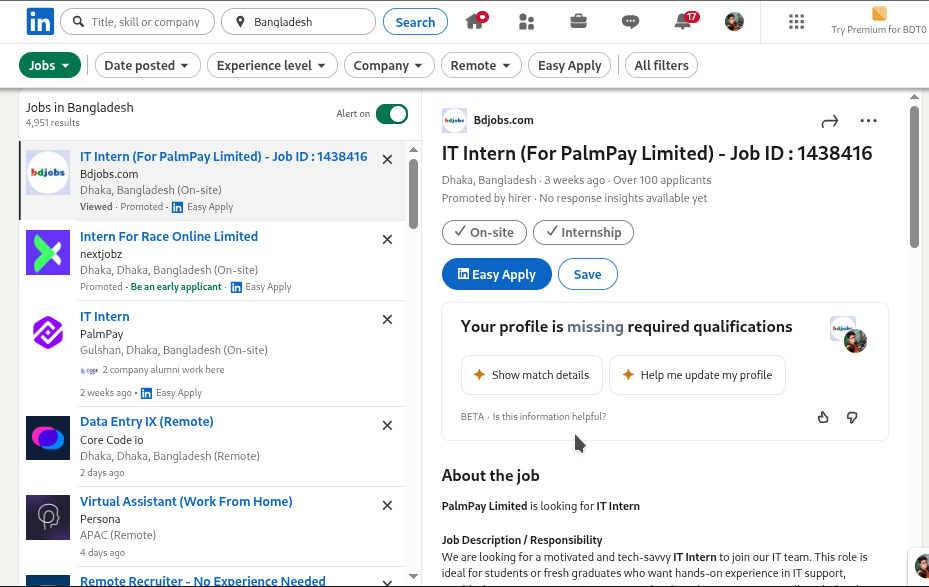
\includegraphics[width=0.85\linewidth]{./images/001LinkedIn.png} % image scale = 0.5 of line width
		\captionof{figure}{LinkedIn Internship Search}
	\end{center}
\\
	The biggest platform is for students is LinkedIn. LinkedIn\cite{linkedin} require students to spend more time either self promoting on the platform and connection building over what actually matters which is skill building and preparing for the job or a long a tedious time filtering through irrelevant job posts that do not match their qualifications or interests. 
	
	\begin{center}
		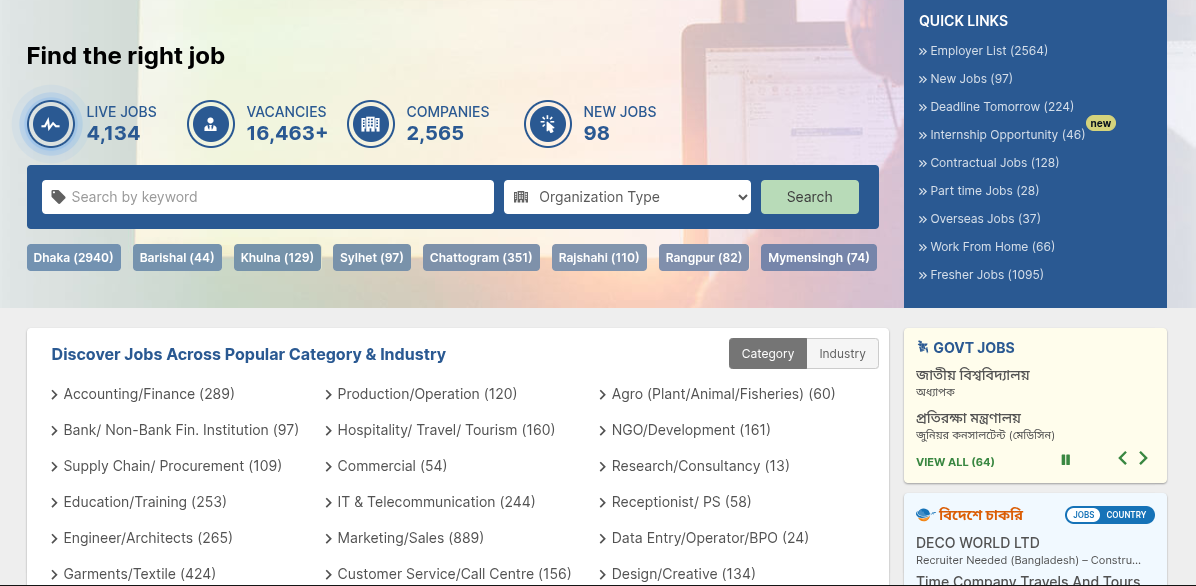
\includegraphics[width=0.85\linewidth]{./images/002bdjobs.png} % image scale = 0.5 of line width
		\captionof{figure}{Bdjobs\cite{bdjobs} website page}
	\end{center}
	\\
	Bdjobs\cite{bdjobs} on the other hand does not have that same problem as LinkedIn but it lacks various listings and almost all the listings are for full time jobs or experienced hires only. This makes it very hard for students to find internships or entry level jobs on the platform. And for the few listings that are for internships or entry level jobs, they are often buried under a lot of other irrelevant listings making it hard for students to find them and most of them are even ghost listings specifically tailored for pre seleceted or referred candidates only. 
\\
\\ 
\\
	While you may think this is the only problem that students face when looking for internships or entry level jobs, there are other and one specially notable nowadays is ghost job listings\cite{bmutasim_ghost_jobs}. While LinkedIn\cite{linkedin} solves this problem in some extent by allowing users to report fake job listing and its social media like structure helps users to identify fake listings through comments and reviews from other users, Bdjobs\cite{bdjobs} lacks such features making it hard for students to identify fake listings. This leads to students wasting their time and effort applying for fake listings only to find out later that they are not real. This not only wastes their time but also demotivates them from applying for other listings in the future.
\\
\\
\\
	This means HR of various companies gives out these ghost job listing in bdjobs \cite{bmutasim_ghost_jobs} and makes the job market look better than it actually is. This creates a false sense of hope for students and fresh graduates who are looking for internships or entry level jobs. They end up applying for these ghost listings and wasting their time and effort only to find out later that they are not real. This not only wastes their time but also demotivates them from applying for other listings in the future.

	
	\section{Motivation}
	The problems we have identified forms the core motivation for developing InternNova. As we have discovered, Bangladeshi students and fresh graduates struggle significantly with finding suitable internship and entry-level job opportunities due to several critical challenges:
	\\
\\
	\textbf{1. Platforms Problems:} Platforms like LinkedIn\cite{linkedin} and Bdjobs\cite{bdjobs} are not optimized for students seeking their first opportunities. LinkedIn requires extensive time investment in self-promotion and networking rather than allowing students to focus on skill development. On the other hand, Bdjobs\cite{bdjobs} doesnt have enough internship and junior-level listings for the job market, making it difficult for students to find relevant opportunities.
	\\
\\
	\textbf{2. Ghost Job Listings:} A big problem in the Bangladesh job market is the number of ghost job listings\cite{bmutasim_ghost_jobs} by some companies to for extended market popularity and social media relevence. Companies post fake positions to inflate their market appearance. These listings waste students' time and effort. More importantly, they undermine student motivation and confidence in the job search process. Bdjobs\cite{bdjobs} is one of the biggest victim of this problem due to the lack of any identification and prevention mechanisms for such fraudulent postings.
	\\
\\
	\textbf{3. Information Asymmetry:} Students don't have access information about companies, internship positions, requirements, and realistic expectations. This information gap stops them from making decisions about which opportunities align with their skills and career aspirations\cite{jiang_information_asymmetry}.
	\\
\\
	\textbf{4. Ghosting After Interviews:} One of the most frustrating experiences for students is when employers ghost them after interviews or any point throughout the application process. Research shows that 61\% of job seekers experience post-interview ghosting, with this rate increasing by 9 percentage points since early 2024\cite{ghosting_index_2025}. Without any communication or feedback, students are left uncertain about their skills and status and thus gets discouraged from future applications. This unprofessional behavior from the companies damages the student experience and creates a cycle of frustration and demotivation. The problem is staggaringly high in Bangladesh where most platforms lack accountability mechanisms to address employment ghosting.
	\\
\\
	\textbf{5. Lack of Feedback from Interviews:} We are already at the point that we dont even receive a rejection letter anymore. So when students receive rejection, also receiving any kinds of constructive feedback is a big dream at this point. Several studies indicate that 75\% of job applications receive zero response from employers\cite{ghosting_index_2025}, leaving candidates with no information about their application status let alone areas needing improvement. This statistics is almost at a full 100\% for Bangladesh unless the candidate have previous network from which they can get the feedback. This prevents students from learning, growing, and refining their interview skills for future opportunities. Students are left guessing what went wrong and how to improve, resulting in an average \textbf{Candidate Time Tax} of approximately 47 hours wasted per job search on ghosted processes\cite{ghosting_index_2025}.
	\\
\\
	These challenges inspired us to create InternNova, a complete platform specifically designed to address the unique needs of Bangladeshi students seeking internships and entry-level positions. By solving these problems one by one we can slowly empower students to navigate the job market more effectively and achieve their career aspirations.
	
	\section{Objectives}
	In our project we have two kinds of objectives, Social and Technical. The social objectives are, 
	\begin{itemize}
		\item To create a trustworthy platform that connects students with genuine internship and entry-level job opportunities, reducing the prevalence of ghost listings.
		\item To empower students with verified information about companies and positions, enabling them to make informed career decisions.
		\item To foster transparency and accountability in the hiring process by implementing mechanisms to address employer ghosting and provide constructive feedback.
	\end{itemize}
	On the other hand some of the technical objectives are,
	\begin{itemize}
		\item To develop a user-friendly web application that allows students to easily search, filter, and apply for internships and entry-level jobs.
		\item To implement a robust backend system that securely manages user data, job listings, and application processes.
		\item To make sure the platform is scalable and can handle a growing number of users and listings over time.
		\item To incorporate security measures to protect user data and ensure privacy.
	\end{itemize}

	\chapter{Literature Review}
	
	\section{Background Study}
	
	\subsection{The Bangladesh Youth Employment Crisis}
	\\
	Bangladesh right now is facing a complicated employment situation where economic growth is not increasing the amount of jobs for its youth population. According to the Centre for Policy Dialogue (CPD), employment growth has not increased in our country despite GDP recovery from various recent(specifically Covid-19) economic crisis, creating what economists like to say as the \textbf{jobless growth}\cite{cpd_employment_2024}. This mismatch between economic growth and employment stagnation affects fresh graduates entering the job market.
	\\
	\\
	The Bangladesh Labour Market in the 2024/2025 economic year reveals alarming statistics about youth unemployment. highlighting a high number of people not in education, employment and training among Bangladeshi youth\cite{bangladesh_labour_market_2024}. This situation is even boosted by low private investment which is generally the biggest job creator of any economy
	\\
	\\
	Another finding from the Bangladesh Institute of Development Studies (BIDS) shows that 28.24\% of National University(One of the largest university in the world in terms of current students) graduates remain unemployed\cite{dhaka_tribune_nu_graduates}. This high unemployment rate among NU graduates breaks open an even deeper structural problem of our country - a curriculum mismatch between what universities teach and what the job market actually needs. Theere are also study that reveals \textbf{university bias} where employers filter CVs to prioritize graduates from top public universities (DU, BUET, IBA) or elite private institutions (NSU, BRAC, AIUB), effectively excluding the almost all of graduates from consideration regardless of their actual capabilities to make interview process easier for them.
	
	\subsection{The Entry-Level Paradox and Salary Exploitation}
	
	The Dhaka Tribune's report on \textbf{Lifting the curse of graduate unemployment} reveals a critical contradiction in Bangladesh's job market - the entry-level paradox\cite{dhaka_tribune_graduate_unemployment}. Employers advertise \textbf{entry-level} positions while simultaneously demanding 2-3 years of prior experience, creating an impossible paradox for fresh graduates. This practice has gone to the point at this moment that students dont even bother to look at the experiece requirements anymore since they have lost their meaning. And this rampant action has given the entry-level word a new meaning which translates to you wont get paid much or you will be exploited.
	\\
	\\
	We also have to add salary exploitation to this crisis as well. Community on the internet suh as r/bangladesh reveal that Bachelor's degree holders are routinely offered salaries of 10,000-15,000 BDT per month for full-time positions\cite{reddit_job_mental_health}. Which is very funny since an average student generally can earn the same amount of money working as a tutor in Dhaka city with about 12-15 hours every mont as a tutor. also in terms of Dhaka's current economic context, these salaries does not even cover rent, daily transportation and meals, making them essentially unlivable wages. there are many cases where students with a Master's degree holder are being offered only 12,000 BDT, demonstrating how qualification levels have become disconnected from compensation.
	
	\subsection{Automation and Closing Traditional Entry Paths}
	
	Dr. Khondaker Golam Moazzem's research for CPD describes that industrial growth in Bangladesh is failing to create jobs due to increasing automation\cite{cpd_industrial_jobs}. The Ready-Made Garment (RMG) sector, traditionally the largest employer of entry-level workers in bangladesh, is experiencing job reduction through advancement in computers. This closes of the \textbf{easy} entry path that previous generations relied upon forces the graduates into more competitive sectors where nepotism and connections play larger roles.
	
	\subsection{Platform-Specific Problems in Bangladesh}
	
	\subsubsection{The Bdjobs \textbf{Black Hole} Phenomenon}
	
	Community discussions across r/bangladesh subreddit consistently shows a pattern unique to Bangladesh's largest job platform, Bdjobs. The \textbf{viewed ghost} phenomenon describes a frustrating experience where application status shows as \textbf{Viewed by Employer} but candidates never receive any subsequent communication\cite{reddit_job_mental_health} from the employers. Unlike some more advanced platforms that send automated rejection emails with automated CV filter, Bangladeshi companies often silently archive applications, a phenomenon known as making a paper plane with the CV.
	\\
	\\
	Multiple users on BDJobs\cite{bdjobs} report that job listings stays marked \textbf{active} long after positions are filled with candidates and generally does not shows any application deadline, not for genuine hiring purposes but primarily for data collection\cite{bdjobs_optimization_video} by the companies. This practice wastes candidates' time and creates a false sense hope in an already difficult job market. Shafiul Azam Shakil's analysis\cite{bdjobs_optimization_video} of common Bdjobs mistakes shows the need for platform-specific optimization strategies that shouldn't be necessary if the platform functioned transparently.
	
	\subsubsection{LinkedIn Bangladesh's Content Problem}
	
	While LinkedIn functions in the LinkedIn are relatively well in Western contexts, its Bangladesh the same process hurts the candidates in a different way. Job seekers almost always complain that feeds are dominated by copied or ai generated motivational content and self-promotional posts rather than genuine hiring opportunities\cite{linkedin}. and the cherry on top is that, the \textbf{Easy Apply} feature often proves deceptive - many local companies enable this functionality but never check those application inboxes, preferring candidates who make direct contact via email or phone calls.
	
	\subsubsection{Facebook and Telegram Scam Ecosystem}
	
	One of the most dangarous of Bangladesh's job market is the rampant scams on the more informal platforms. Fraud listings, particularly for data entry or airport jobs, request \textbf{security money or application fee} ranging from 500-2,000 BDT via mobile banking services like bKash or Nagad for supposed \textbf{registration} or \textbf{ID card} fees. Many legitimate employers first started this allication fee to reduce the number of fake applications in their job circulars. But now this is getting used by scammers to get the application fee from desperate students looking for employment. This has gotten so bad that now legitimate companies never request any money from job applicants at any point of the job application and examination process, making asking any application a red flag to avoid.
	
	\subsection{The 6-Day Work Week Deception}
	
	Communities on the internet reveal a systematic pattern of dishonesty about work life culture\cite{reddit_job_frustration} in Bangladesh. Job listings almost always advertise \textbf{5 days a week} working arrangements, but during final interviews or after joining, employees discover that they must work Saturdays or sometimes even fridays before any large holidays as well - this is the classic the \textbf{6-day trap.} This bait-and-switch reveals the transparency problems in Bangladesh's companies where these false problems are used to attract good candidates.
	
	\subsection{Internship Exploitation and \textbf{Coffee Culture}}
	
	Most local internships in Bangladesh are completely unpaid, or if it is even compensated, most offer only the very minimal \textbf{transport allowances} of 3,000-5,000 BDT. Other than the extremely low pay there is a systematic misuse of interns. Multiple reports indicate interns are often assigned menial tasks like fetching tea, making photocopies, and running personal errands for senior staff rather than receiving actual professional training and skill development which was the main target of the internships for the students. This culture undermines the educational purpose of internships and exploits students' desperate need for credentials for their career improvement.
	
	\subsection{Mental Health Impact}
	
	When we sum up all the effects of these barriers, this creates severe mental health consequences for the youths. Discussions on r/bangladesh titled \textbf{Job Searching and Mental State} and \textbf{No luck finding a job leading to insanity} shows job seekers are suffuring from severe depression, anxiety, and hopelessness\cite{reddit_job_mental_health}\cite{reddit_civil_engineer}. The combination of ghosting, nepotism, exploitation, and false promises creates a psychologically damaging experience that extends far beyond mere economic hardship.
	
	\subsection{International Context: The Ghosting Epidemic}
	
	Bangladesh is not the unique here in the ghosting problem from the employers, professional ghosting has become a global crisis. The 2025 Ghosting Index, analyzing over 50 studies worldwide, found that 61\% of job seekers experience post-interview ghosting, with this rate has increased by 9\% since early 2024\cite{ghosting_index_2025}. To rub salt to the injury, 75\% of job applications receive zero response from employers globally, creating an average \textbf{Candidate Time Tax} of 47 hours wasted per job search.
	\\
	\\
	This international context reveals that while Bangladesh's problems have local characteristics (nepotism, university bias, application fee scams), the fundamental breakdown in hiring communication is a global issue. However, the lack of accountability in Bangladesh for the local problems should be accounted for. and we should implement legal, technical mechanisms and worker protections that has solved some problems in other market and implement the solutions that have worked historically here to the situation mentally bearable for Bangladeshi job seekers.
	
	\subsection{The Skills Mismatch}
	
	Research by CPD and BIDS consistently identifies a fundamental \textbf{skills mismatch} - universities teaching theoretical knowledge while employers demand practical software and soft skills\cite{cpd_employment_2024}\cite{dhaka_tribune_nu_graduates}. This gap means even qualified graduates struggle to demonstrate job-ready capabilities, further disadvantaging them in an already hostile job market. The curriculum disconnect particularly affects National University graduates, who represent the majority of Bangladesh's higher education output but receive the least market recognition.
	
	\section{Our Solution}
	All of these problems are technically not solvable by one singular project using any specific systems or any specific math or systems thanks to the good old rule of economics, \textbf{When a measure becomes a target, it ceases to be a good measure}. But we have decided to create our own job platform \textbf{InternNova} where we are attempting to solve as many as problems as possible.
	\\
	
	Some of the key problems which we are targeting to solve are,
	\begin{itemize}
		\item \textbf{Platform Problems:} We have created a user friendly platform which has significantly less noise and complexity compared to platform like Bdjobs\cite{bdjobs} which although seems to give excellent choices and options for filtering and other systems but in reality makes it harder for students who are new to this platform, find internships or entry level jobs. On the other hand, LinkedIn\cite{linkedin} although is a great platform for professionals but for students looking for internships or entry level jobs, The amount of self promotion and marketing that is required for 
		\item \textbf{Ghost Job Listings:} We have assigned a very strict verfication process for companies who want to post job listings on our platform. This is solved using multiple steps. Firstly we have made sure that no company can post a job listing without having a complete profile. We have done this to make it as much difficult as possible for botnneckers to create fake company profiles and overflow our platform with fake job listings. This also makes it easier for our own logisitcs as well since we can verify the company data and cross validate informations. The second step is the manual verification of the companies with the admin team. The admin team will verify the company data and make sure that the company  is legitimate. Although this is a time consuming process and this can make many companies frustrated enoough to not use our platform, the admin team will only ban companies who are found to create fake job listing or found to have a bad history of ghosting candidates or any other unprofessional behavior. This banning system will allow us to maintain a high quality of job listings on our platform without making the verification process too strict for legitimate companies.
		\item \textbf{User or Candidate Verification:} Although it may seem very strict we have made sure that the same level of restrictions is applied to the candidates as well. In other word, a normal candidate cannot just create an account and start applying for jobs. The candidate has to complete their profile and then verify their identity to start using our platform. Since most of our target audience are students, we can verify the identity of the candidates using their various levels of certifications such as SSC, HSC, Diploma, Bachelors and Masters. SSC and HSC results can easily be verified using the official government websites and for higher levels of education, we can keep the verification process less stringent and then only ban the users when found to be misusing the platform. This verification process will stop bots and fake users from flooding applications to job listings and thus will make it easier for the companies to find genuine candidates.
		\item \textbf{Application Tracking and Feedback System:} We have created an application tracking system where candidates can track the status of their applications in real time. This tracking system will be connected to the company's dashboard where the HR of that company can update the status of the job listing with various status such as \textbf{Pending}, \textbf{Accepted}, \textbf{Rejected} or other status. This solves one of the biggest problems of ghosting the applicants at any point of the application process. So applicants can move on to another opportunity without wasting their time waiting for a response from the company. 
 	\end{itemize}
	\\
	\\
	Unfortunately, due to both human reasons, time resoureces available to us and some technical limitations we could not solve all the problems with this project. Such as the nepotism problems, the 6 day work week deception problems and the internship exploitation problems. These problems are created due to the bad cultural and social behavior or the people and companies of Bangladesh. We can also ban these companies from our platform but that will not solve the problems created by people as the people causing these problems can also move to other companies and contineue the same behaviors. So we had to take these problems our of the scope of our project. 
	\\

	\section{Functional Requirements}
	The functional requiremments of our projects can be divided into various roles such as Admin, Company, Candidate and the system in general. The system is the main contributor and will have to do the following tasks depending on the roles of the users whom the system is interacting with, 
	\begin{itemize}
		\item \textbf{Admin:} The admin will have the highest level of access to the system. The admin will be able to manage the companies and candidates on the platform such as banning or deleting users job listings or even company accouunts. The admin will also be able to verify the companies and candidates. This power makes the admin account and interaection endpoints very important and we have to make sure to keep it protected from any kind of unauthorized access. so functionally the system have to, 
		\begin{itemize}
			\item Verify that the user is admin before allowing access to admin endpoints.
			\item Log all admin activities for auditing purposes for recovering any unauthorized temparing.
			\item Provide a dashboard for admin to manage companies and candidates.
		\end{itemize}
		\item \textbf{Company:} The companies are the second most privilaged roles in our platform. The companies will be able to post job listings, manage their company profile and view the applications for their job listings. So functionally the system have to,
		\begin{itemize}
			\item Verify that the user is a company before allowing access to any company endpoints.
			\item Allow companies with complete informations to create and manage their job listings. 
			\item Allow companies the management access to the circulars and applications for their job listings.
		\end{itemize}
		\item \textbf{Candidate:} The candidates are the main users of our platform. The candidates will be able to create their profiles, search for job listings, apply for job listings and track their applications. So functionally the system have to,
		\begin{itemize}
			\item The system have to make sure that the user data is confidential and secure to all other users including companies and admins unless the user have applied to a job listing of that company.
		\end{itemize}
	\end{itemize}

	\chapter{Methodology}
	\section{Application Flow}
	If we want to simplify the application flow of our project, we can divide it into either by roles or by the process itself. By roles the most important process or data flow is the user authentication and authorization process. This includes registration, login, passoword resetting, email verification and other similar processes. On the other hand when we want to talk about the process flow, the most important process is the application lifecycle which is comprised of job listing creationm job searching, application process of the candidates, application tracking, interview, hiring and circular closing.
	\\

	\subsection{User Authentication and Authorization Flow}
	The user authentication and authorization is the user management system is the heart and soul of our project. We must have an user management system which is secure and reliable to make sure that the user data is protected and the users can trust while we also have proper access control system in place. 
	\\
	\\
	In our project we have used a dual-token(Access + Refresh) JWT method based authentication and authorization system. There is a short lived access token which lasts for 15 minutes and a logn lived access token that lasts for 7 days. The access token is for user authentication and authorization for accessing protected endpoints and the refresh token is for getting a new access token when the old one expires. This method is more secure than the traditional session based authentication system as we do not have to store any session data on the server side and we can also make sure that the user data is protected from any kind of unauthorized access. While adding the fact we have a no storing passoword policy where we do not even take the passwords to any database and we only store the salted bcrypt hashed password which is considered one of the most secure hashing algorithms available today.
	\\
	\\
	We also have added a Email verification system with a 10 minute expiring 6 digits randomly generated OTP key to make sure that the user is a legitimate user and the email is valid. This also helps us to prevent bot accounts to mass register on our platform. 
	\\
	\\
	This is a complex system with a nuance that the user have to log in to the websitre every 15 minutes. But this is a trade off we had to make to ensure the security of the user data and the platform as a whole. 
	\begin{center}
		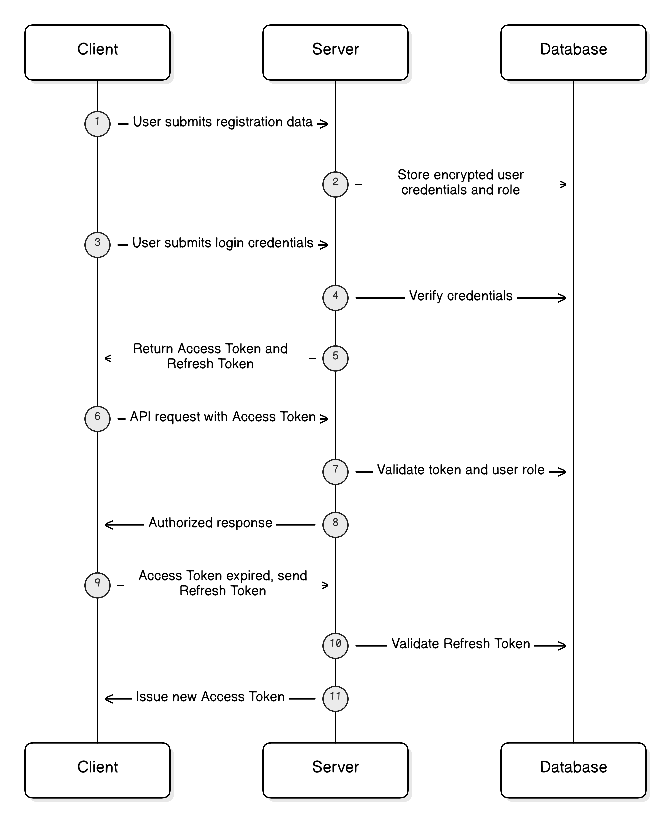
\includegraphics[width=0.85\linewidth]{./images/diagram-01.png} % image scale = 0.5 of line width
		\captionof{figure}{Application Flow Diagram of user authentication and authorization}
	\end{center}
	\\
	The Role-Based accesss control we have implemented have two layers of security for both front end and back end. The front end component \textbf{ProtectedRoute} limits user interface access and redering of the elements of baed on the user role. On the other hand the backend component \textbf{authMiddleware} and \textbf{roleMiddleware} validates JWT signatures to strictly restricts user role. Combining the two layers creates a strong security system for the appliction.
	\\
	\subsection{Application Lifecycle Flow}
	The application lifecycle is the main process of our project. This process starts with creating a circular by a company and ends with closing of that said circular after the hiring process. 

	\begin{center}
		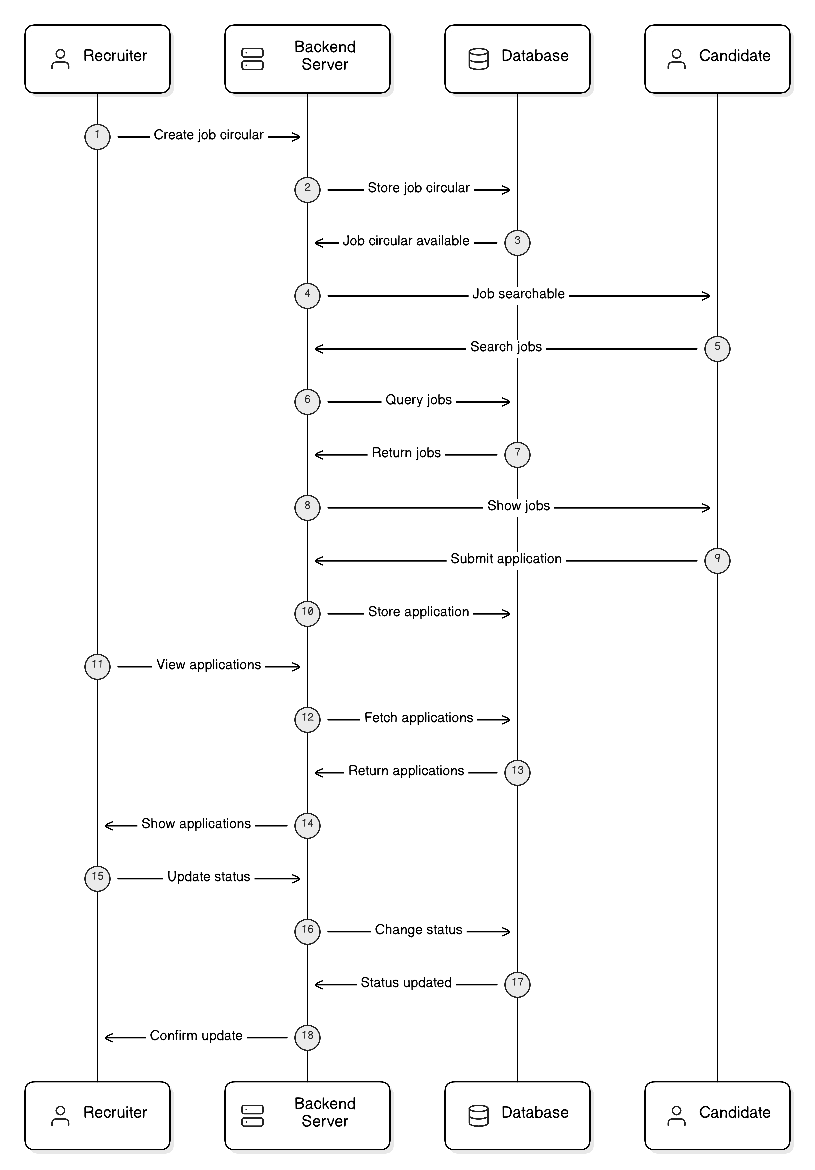
\includegraphics[width=0.8\linewidth]{./images/diagram-02.png} % image scale = 0.5 of line width
		\captionof{figure}{Application Lifecycle Flow Diagram}
	\end{center}
	The Application lifecycle starts with a company creating a job listing or circular on our platform. The company have to have a complete profile and verified account to be able to create a job listing. Once the job listing is created, it will be visible to all the candidates on the platform. The candidates can then search for job listings using various filters and apply for the job listings they are interested in. Once the candidate applies for a job listing, the application will be sent to the company for review. The company can then review the applications and update the status of the applications such as \textbf{Pending}, \textbf{Accepted}, \textbf{Rejected} or other status. The candidates can then track the status of their applications in real time using our application tracking system. Once the hiring process is complete, the company can close the circular and the job listing will no longer be visible to the candidates.

	\section{Function and Modules}
	Our Project have multiple user types and with each user and functionality we have various methods or endpoints. But by definition we have divided our modules on the basis of both tasks and controllers. So the controllers and some example of their functions or endpoints are,

	\begin{itemize}
		\item Authentication Module (\texttt{/api/auth})
		\begin{center}
		\footnotesize
		\begin{tabularx}{\linewidth}{|l|l|X|l|}
		\hline
		\textbf{Method} & \textbf{Endpoint} & \textbf{Description} & \textbf{Access} \\\hline
		POST & \texttt{/register} & Register a new user (Candidate/Recruiter) & Public \\\hline
		POST & \texttt{/login} & Authenticate user \& obtain tokens & Public \\\hline
		POST & \texttt{/refresh-token} & Refresh expired access token & Public \\\hline
		GET & \texttt{/me} & Get current user context & Private \\\hline
		POST & \texttt{/logout} & Logout user & Private \\\hline
		POST & \texttt{/forgot-password} & Initiate password reset & Public \\\hline
		POST & \texttt{/reset-password} & Complete password reset & Public \\\hline
		POST & \texttt{/verify-email} & Send verification OTP to user's email & Public \\\hline
		POST & \texttt{/verify-otp} & Verify OTP and activate account & Public \\\hline
		POST & \texttt{/resend-otp} & Resend verification OTP (rate-limited) & Public \\\hline
		\end{tabularx}
		\captionof{table}{Authentication Module Endpoints}
		\end{center}

		\item Jobs Module (\texttt{/api/jobs})
		\begin{center}
		\footnotesize
		\begin{tabularx}{\linewidth}{|l|l|X|l|}
		\hline
		\textbf{Method} & \textbf{Endpoint} & \textbf{Description} & \textbf{Access} \\\hline
		POST & \texttt{/} & Create a new job listing & Recruiter \\\hline
		GET & \texttt{/} & List jobs (filters: keyword, location, etc.) & Public \\\hline
		GET & \texttt{/:id} & Get single job details & Public \\\hline
		PUT & \texttt{/:id} & Update job details & Recruiter (Owner) \\\hline
		DELETE & \texttt{/:id} & Delete a job & Recruiter (Owner) \\\hline
		PATCH & \texttt{/:id/status} & Update status (active/paused/closed) & Recruiter (Owner) \\\hline
		GET & \texttt{/recruiter/my-jobs} & Get jobs posted by current recruiter & Recruiter \\\hline
		GET & \texttt{/recruiter/stats} & Get job statistics & Recruiter \\\hline
		\end{tabularx}
		\captionof{table}{Jobs Module Endpoints}
		\end{center}
		\newpage

		\item Companies Module (\texttt{/api/companies})
		\begin{center}
		\footnotesize
		\begin{tabularx}{\linewidth}{|l|l|X|l|}
		\hline
		\textbf{Method} & \textbf{Endpoint} & \textbf{Description} & \textbf{Access} \\\hline
		GET & \texttt{/} & List all companies & Public \\\hline
		GET & \texttt{/:id} & Get company public profile & Public \\\hline
		GET & \texttt{/:id/jobs} & Get jobs for a specific company & Public \\\hline
		GET & \texttt{/me} & Get own company profile & Recruiter \\\hline
		PATCH & \texttt{/me} & Update company profile \& logo & Recruiter \\\hline
		PATCH & \texttt{/change-password} & Change account password & Recruiter \\\hline
		\end{tabularx}
		\captionof{table}{Companies Module Endpoints}
		\end{center}

		\item Applications Module (\texttt{/api/applications})
		\begin{center}
		\footnotesize
		\begin{tabularx}{\linewidth}{|l|l|X|l|}
		\hline
		\textbf{Method} & \textbf{Endpoint} & \textbf{Description} & \textbf{Access} \\\hline
		POST & \texttt{/apply} & Submit a job application & Candidate \\\hline
		GET & \texttt{/my} & List own applications & Candidate \\\hline
		GET & \texttt{/job/:jobId} & View applicants for a specific job & Recruiter \\\hline
		PUT & \texttt{/:id/status} & Update application status (shortlist/reject) & Recruiter \\\hline
		\end{tabularx}
		\captionof{table}{Applications Module Endpoints}
		\end{center}

		\item Candidates Module (\texttt{/api/candidates})
		\begin{center}
		\footnotesize
		\begin{tabularx}{\linewidth}{|l|l|X|l|}
		\hline
		\textbf{Method} & \textbf{Endpoint} & \textbf{Description} & \textbf{Access} \\\hline
		GET & \texttt{/me} & Get own candidate profile & Candidate \\\hline
		PUT & \texttt{/me} & Update candidate profile & Candidate \\\hline
		PUT & \texttt{/change-password} & Change account password & Candidate \\\hline
		GET & \texttt{/applied-jobs} & List applied jobs (Detailed) & Candidate \\\hline
		GET & \texttt{/bookmarks} & Get bookmarked jobs & Candidate \\\hline
		POST & \texttt{/bookmarks/:jobId} & Add job to bookmarks & Candidate \\\hline
		DELETE & \texttt{/bookmarks/:jobId} & Remove job from bookmarks & Candidate \\\hline
		\end{tabularx}
		\captionof{table}{Candidates Module Endpoints}
		\end{center}
	\end{itemize}
	All of these modules and their functions combines together to create a complete job platform where companies can post job listings and candidates can apply for those job listings. The system also have various other features such as application tracking, candidate verification, company verification and other features to make sure that the platform is secure and reliable for both companies and candidates.

	\chapter{Design and Implementation}
	\section{User Interface}
	Although our interface is significantly simpler and is less featured compared to other platforms such as Bdjobs\cite{bdjobs} and LinkedIn\cite{linkedin}, we have made sure that our interface is user friendly and easy to use for both companies and candidates. We have used a clean and simple design with a focus on fast information fetching and easy navigation through the website. The main pages of our websites are, 
	\begin{itemize}
		\item \textbf{Navigation pannel : } We have used a simple navigation pannel at the top of the page with the logo at the left side tab menu at the center and the user profile and authentication at the right side.
	\end{itemize}
	\begin{center}
		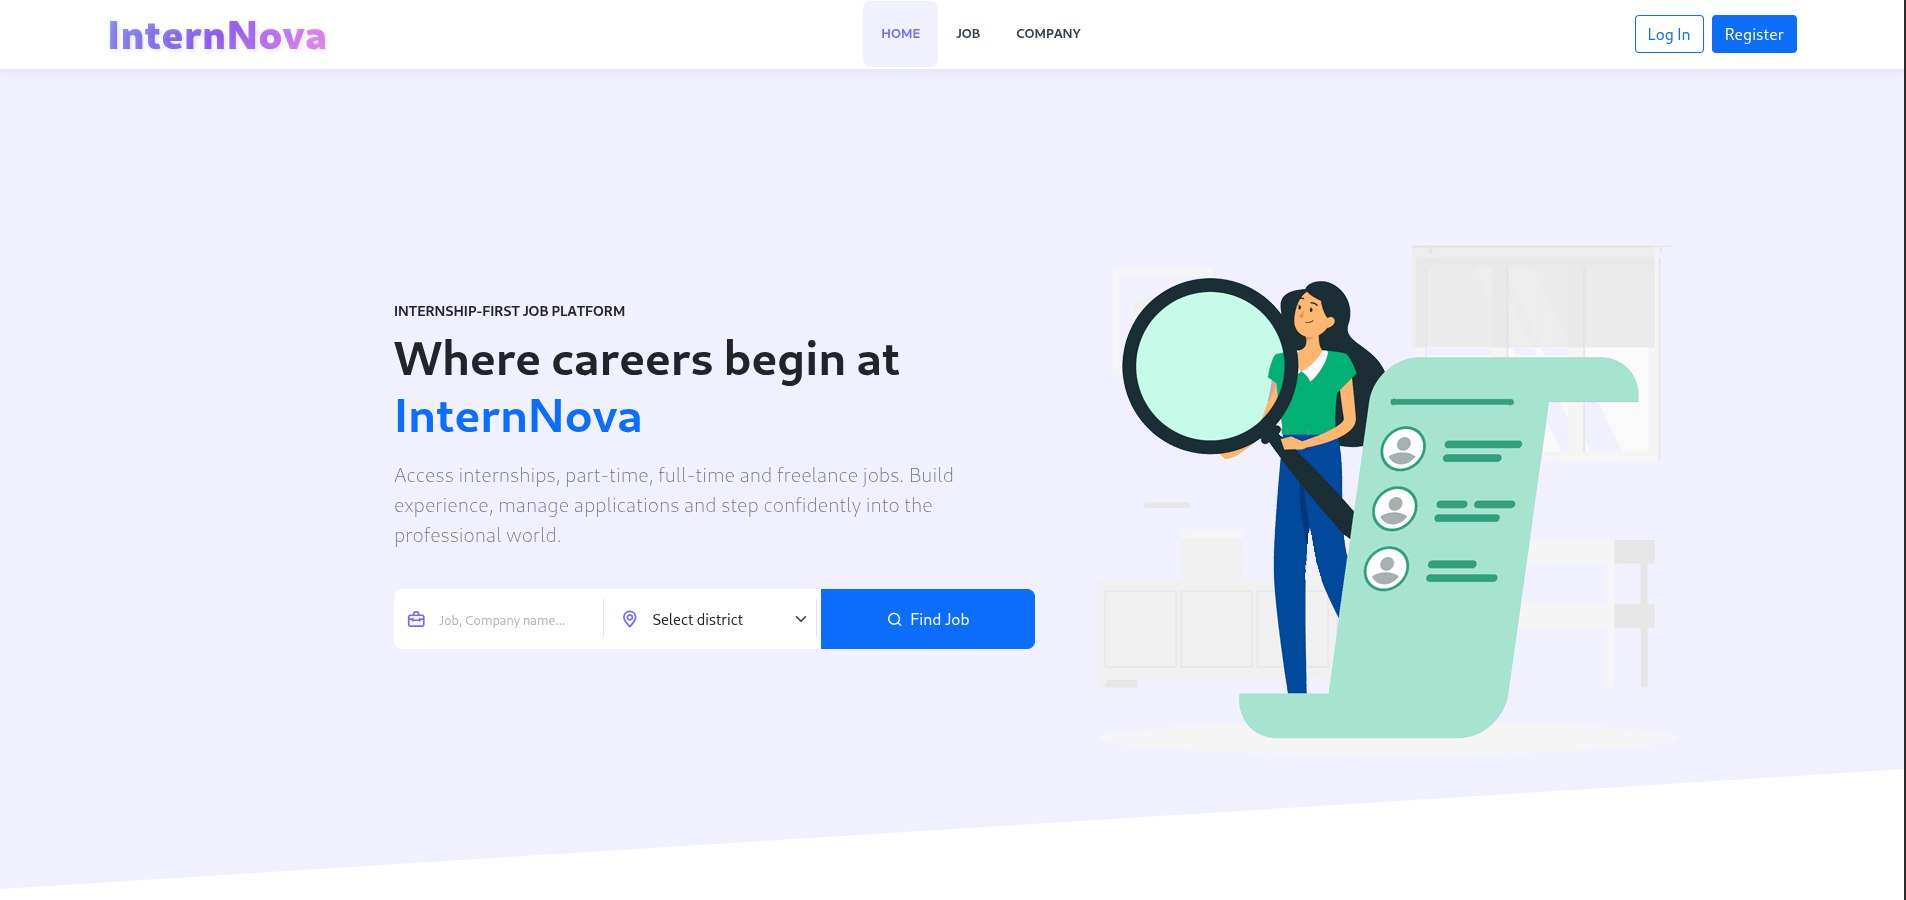
\includegraphics[width=1\linewidth]{./images/interface-01.jpg} % image scale = 0.5 of line width
		\captionof{figure}{Homepage and Navigation Pannel}
	\end{center}
	
	\newpage
	\begin{itemize}
		\item \textbf{Authentication pages : } The user authentication have three pages. Signup page, Login page and Forgot Password page.  
	\end{itemize}
	\begin{center}
		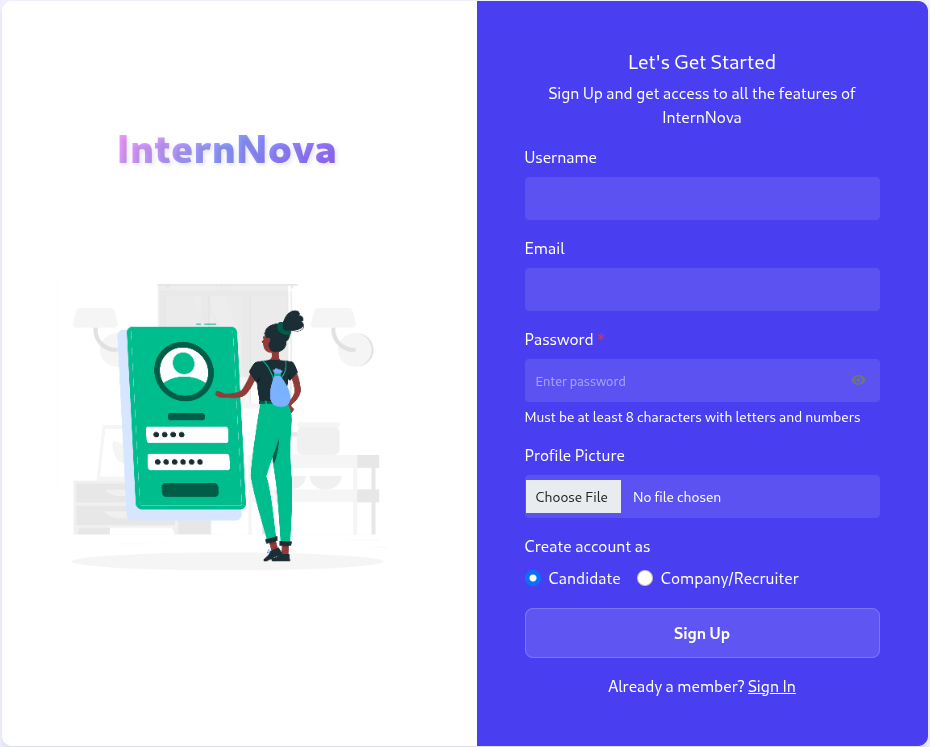
\includegraphics[width=0.9\linewidth]{./images/Screenshot From 2026-01-23 15-15-18.png} % image scale = 0.5 of line width
		\captionof{figure}{User Sign Up page}
	\end{center}
	\begin{center}
		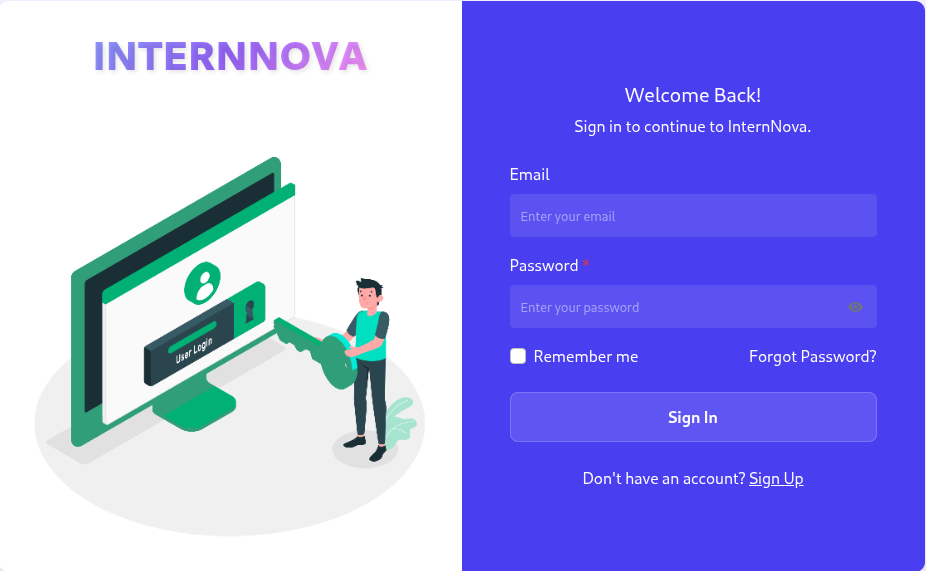
\includegraphics[width=0.9\linewidth]{./images/Screenshot From 2026-01-23 15-14-58.png} % image scale = 0.5 of line width
		\captionof{figure}{User Sign In page}
	\end{center}
	\begin{center}
		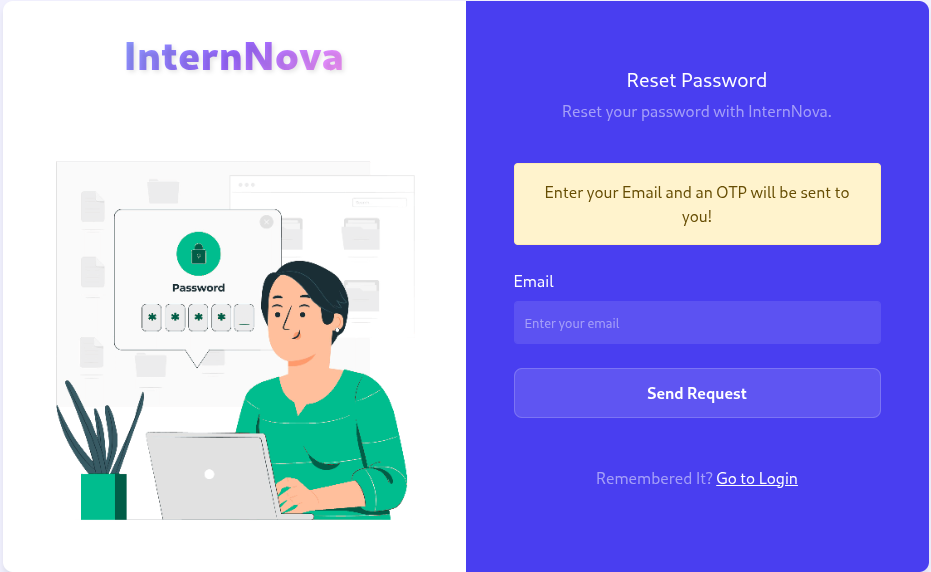
\includegraphics[width=0.9\linewidth]{./images/Screenshot From 2026-01-23 15-15-38.png} % image scale = 0.5 of line width
		\captionof{figure}{Reset Password page}
	\end{center}
	\begin{center}
		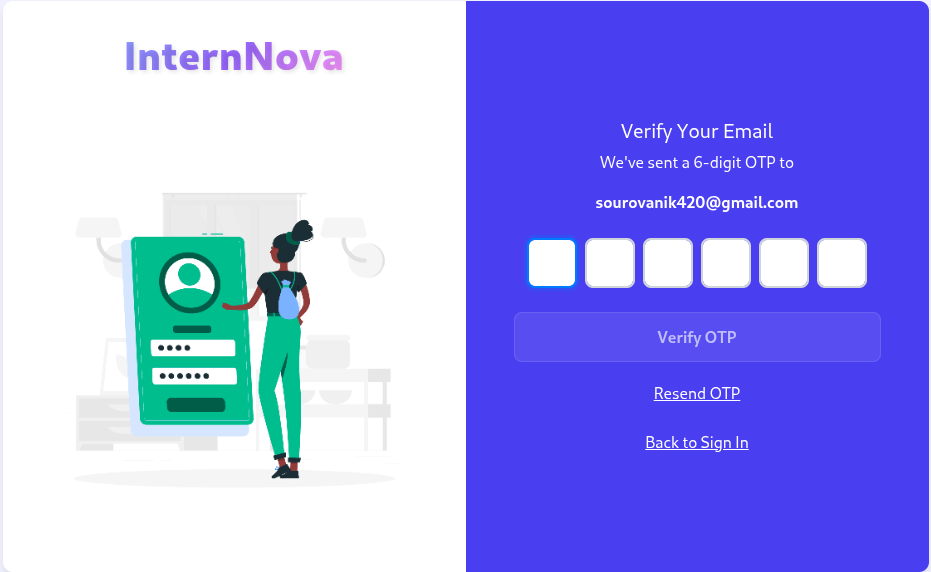
\includegraphics[width=0.9\linewidth]{./images/Screenshot From 2026-01-23 15-16-01.png} % image scale = 0.5 of line width
		\captionof{figure}{Email Verification with OTP page}
	\end{center}
	\begin{center}
		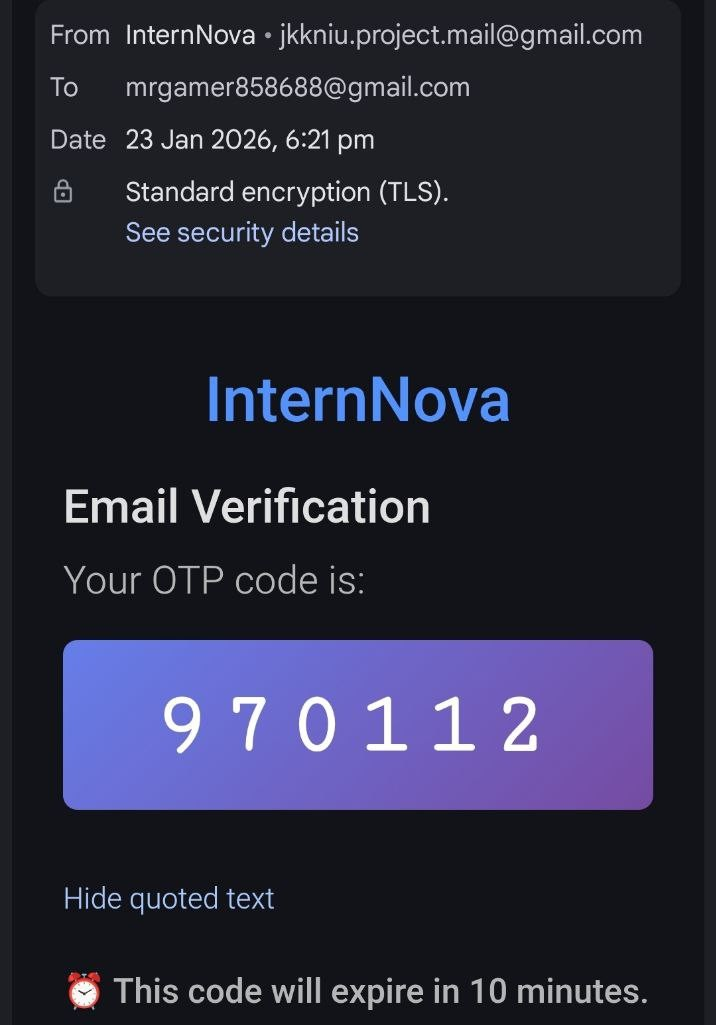
\includegraphics[width=0.5\linewidth]{./images/photo_2026-01-23_20-05-49.jpg} % image scale = 0.5 of line width
		\captionof{figure}{Email with OTP for Email Verification}
	\end{center}
	
	\begin{itemize}
		\item \textbf{Company Profile and menu : } The company profiles and menus are consists of various parts as well. Some of the examples are as shown,
	\end{itemize}
	\begin{center}
		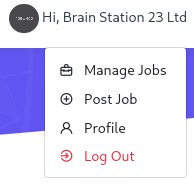
\includegraphics[width=0.5\linewidth]{./images/interface-05.jpg} % image scale = 0.5 of line width
		\captionof{figure}{The Username Dropdown Menu when company is logged in}
	\end{center}
	\begin{center}
		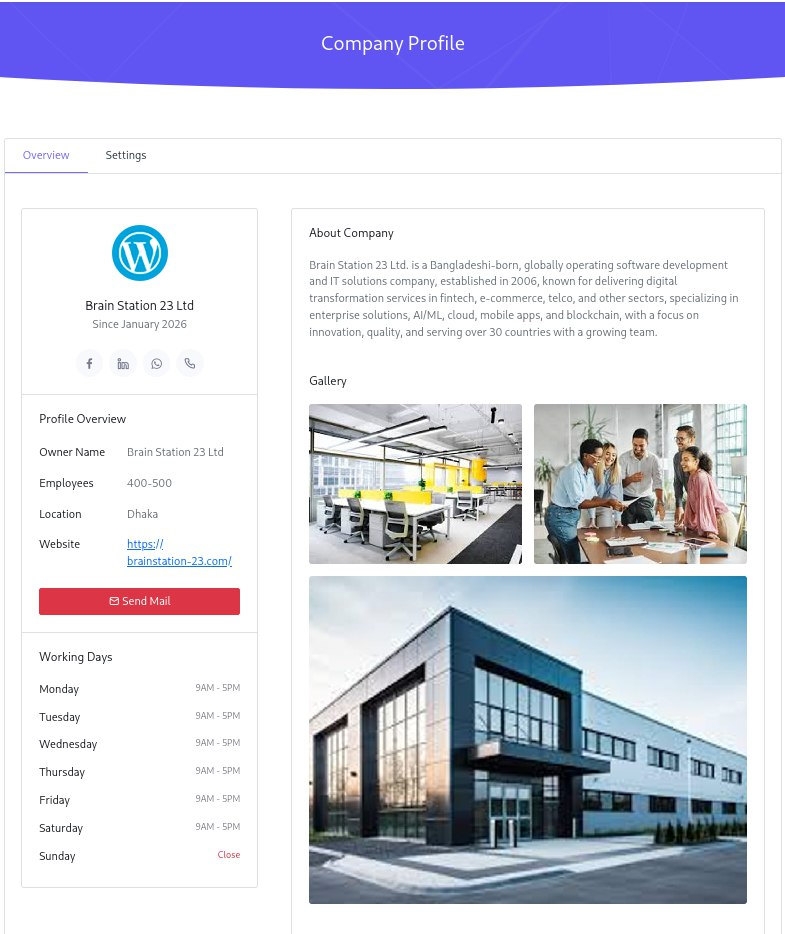
\includegraphics[width=1\linewidth]{./images/interface-06.jpg} % image scale = 0.5 of line width
		\captionof{figure}{The Company Profile page}
	\end{center}
	\begin{center}
		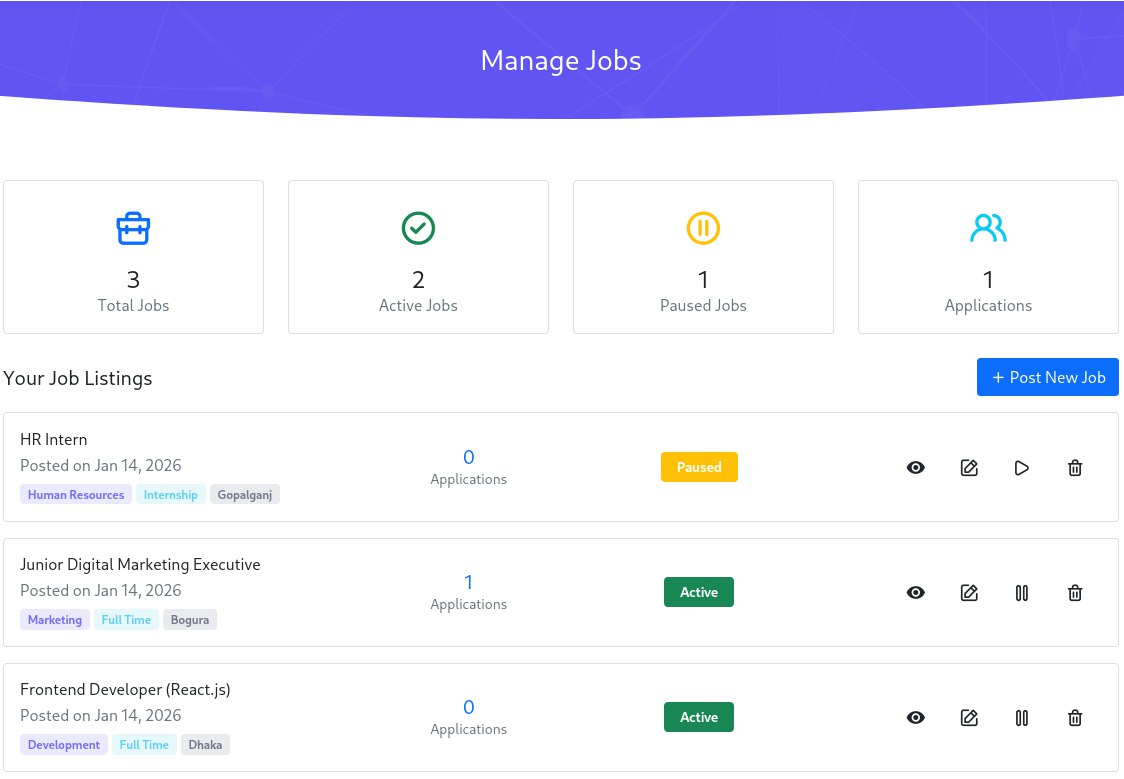
\includegraphics[width=0.9\linewidth]{./images/interface-07.jpg} % image scale = 0.5 of line width
		\captionof{figure}{The Company's page to manage job listings}
	\end{center}
	\begin{center}
		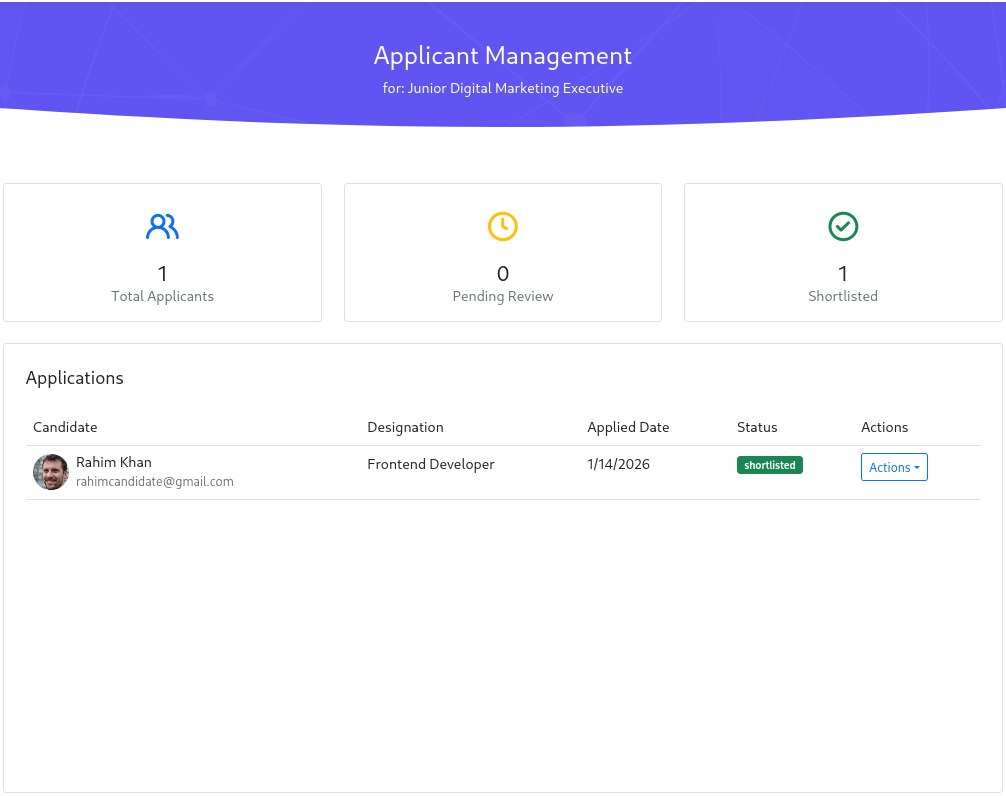
\includegraphics[width=0.9\linewidth]{./images/interface-08.jpg} % image scale = 0.5 of line width
		\captionof{figure}{The Companies page to view applicants for a job listing}
	\end{center}

	\newpage
	\begin{itemize}
		\item \textbf{Candidate Profile and Menu : } The candidates cannot have the same profiles and options but their own custom profiles and menus. Some of the examples are,
	\end{itemize}
	\begin{center}
		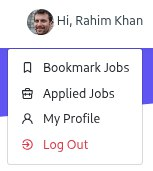
\includegraphics[width=0.5\linewidth]{./images/interface-09.jpg} % image scale = 0.5 of line width
		\captionof{figure}{The Username Dropdown Menu when candidate is logged in}
		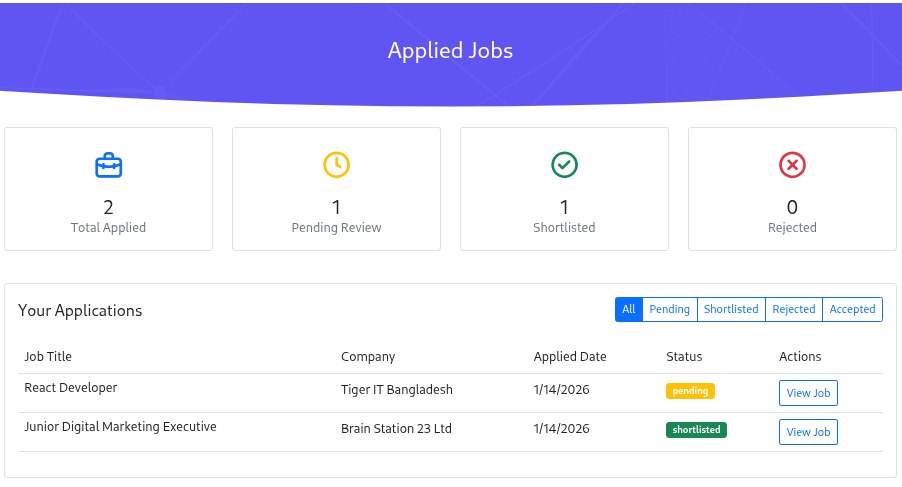
\includegraphics[width=0.9\linewidth]{./images/interface-11.jpg} % image scale = 0.5 of line width
		\captionof{figure}{The Candidate's page to view their applications}
		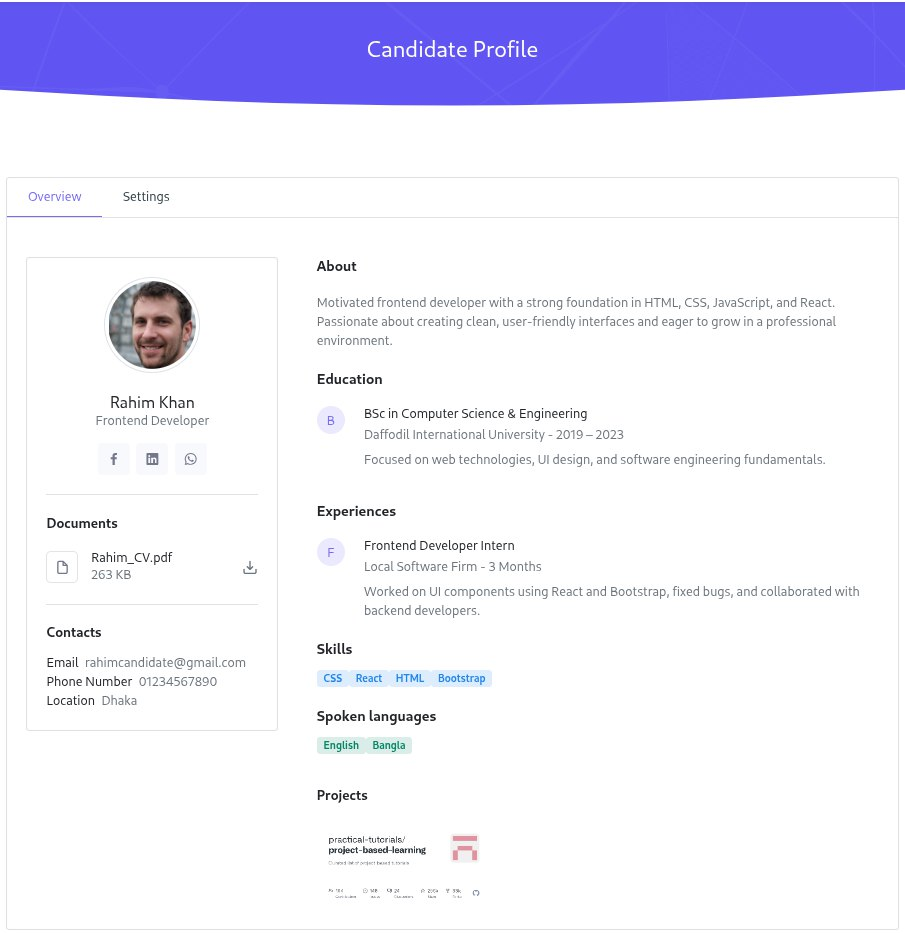
\includegraphics[width=1\linewidth]{./images/interface-10.jpg} % image scale = 0.5 of line width
		\captionof{figure}{The Candidate's Profile page}
		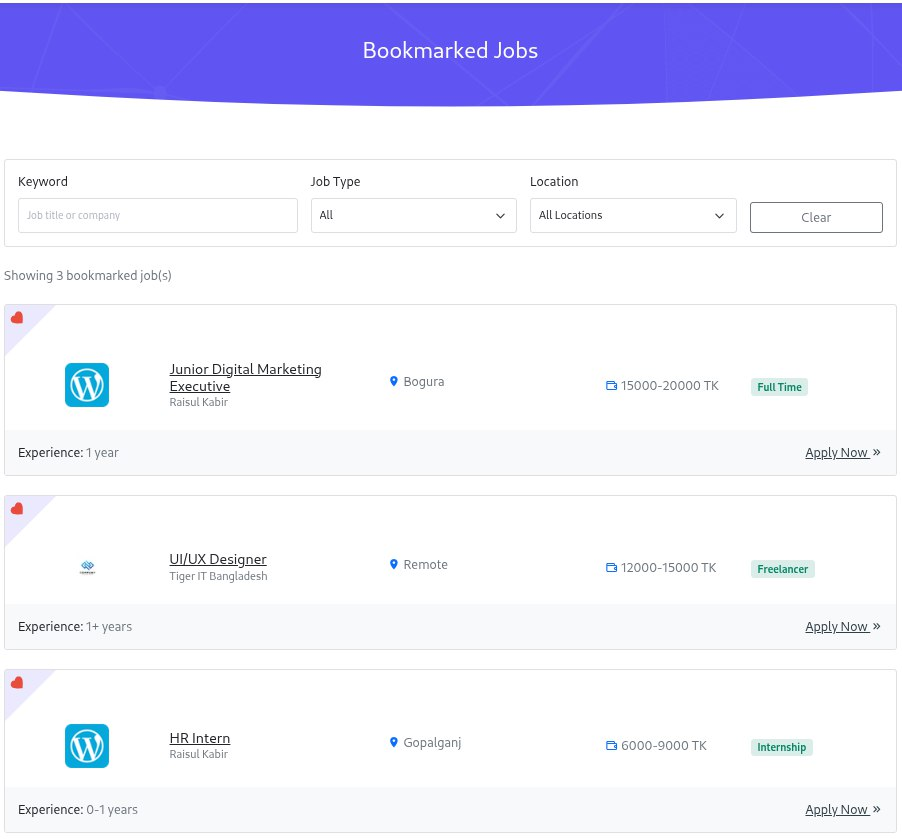
\includegraphics[width=0.9\linewidth]{./images/interface-12.jpg} % image scale = 0.5 of line width
		\captionof{	figure}{The Candidate's page to view and manage bookmarked jobs}
	\end{center}

	\newpage
	\begin{itemize}
		\item \textbf{Browse Jobs : } This is available for all types of users including non logged in users as well.
	\end{itemize}
	\begin{center}
		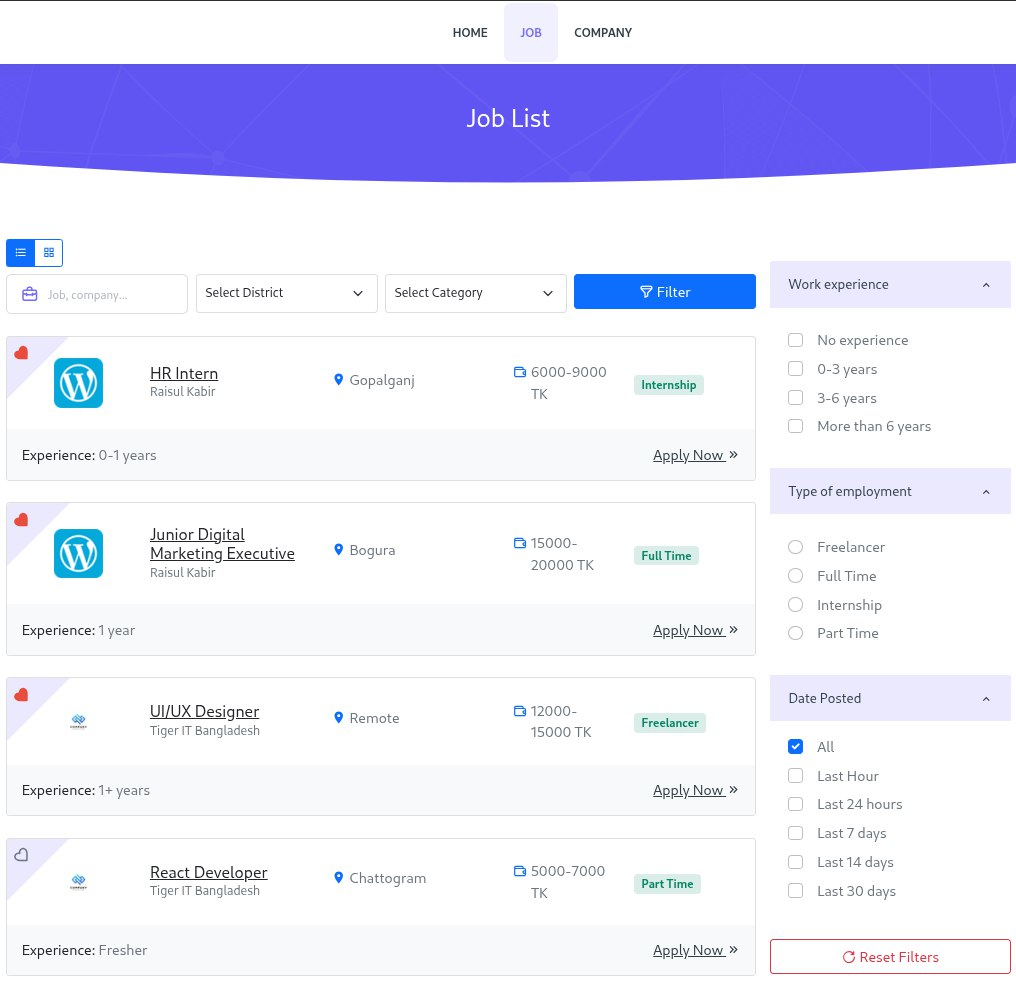
\includegraphics[width=1\linewidth]{./images/interface-13.jpg} % image scale = 0.5 of line width
		\captionof{figure}{The Browse Jobs page with various filters and search options}
	\end{center}

	\newpage
	\begin{itemize}
		\item \textbf{Browse Companies : } This is also available for all types of users including non logged in users as well.
	\end{itemize}
	\begin{center}
		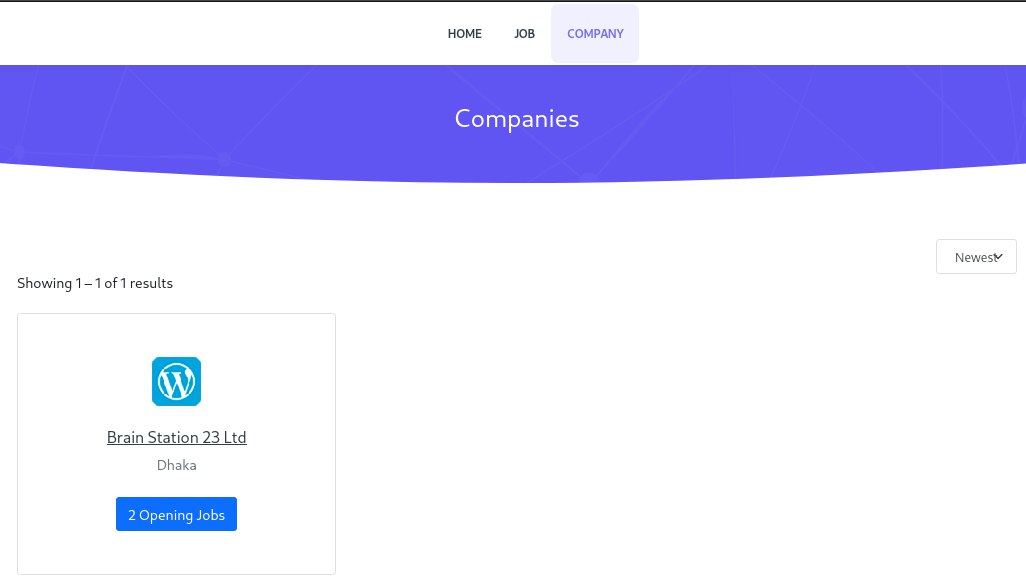
\includegraphics[width=1\linewidth]{./images/interface-14.jpg} % image scale = 0.5 of line width
		\captionof{figure}{The Browse Companies page with various filters and search options}
	\end{center}


	\section{Security Measures and Vulnerabilities Prevention}
	We have heavily enforced security measures in our project to the point we can even divide our security and vulnerability preventions into the following classes, 
	\begin{enumerate}
		\item \textbf{Authentication and Session Management:} Our application InternNova has a robust stateless authentication and session management system with the following security measures,
		\begin{itemize}
			\item Dual-token JWT system with a short access token and long refresh token for obtaining the access tokens
			\item Secure password storage using salted bcrypt hashing
			\item The refresh tokens are stored in httponly cookies to prevent Client Side Scripting (XSS) attacks.
			\item The refresh tokens are rotated to prevent token theft and reuse attacks.
			\item Email verification 10 minute expiring OTPs (sent to user email) for account activation.
		\end{itemize}
		\item \textbf{Authorization and access control:} We have implemented a role based access control system here with the following security measures to prevent unauthorized access to protected endpoints using Middleware Enforcement,
		\begin{itemize}
			\item authMiddleware that verifies the JWT signature and extracts user context from the token.
			\item roleMiddleware that checks the user role from the token and restricts access based on required roles for each endpoint.
		\end{itemize}
		With these the other jobController and applicationController verifies user and ownerships of the data before any modification or deletion.
		\item \textbf{Input validity and data integrity:} All the forms in our applications use express-validator to enforce strict rules preventing invalid or malicious data from entering the system. This prevents Script Injection types attacks such as SQL injection.
		\item \textbf{File upload security:} For file upload one of the biggest risk for any web application is something called reverse shell attack or a virus upload. For image uplaoads we used \textbf{sharp} library to re encode and sanitize the image before storing that in the server.
		\item \textbf{Anti-automation and brute force protection:} We have implemented rete limiting in our authentication endpoints to prevent brute force attacks.
	\end{enumerate}

	\newpage
	\section{Development tools and Environment}
	In the development of InternNova, we have utilized a variety of modern tools and technologies to ensure a robust, scalable, and user-friendly platform. These tools are categorized into frontend, backend, and development/DevOps utilities.

	\subsection{Frontend Development (Client)}
	\begin{center}
	\begin{tabularx}{\linewidth}{|c|l|X|}
	\hline
	\textbf{Logo} & \textbf{Tool Name} & \textbf{Purpose and Reasoning} \\ \hline
	
\includegraphics[height=1cm]{./images/react.png}\captionlistentry[figure]{React Logo} & React\cite{react} & Component-based UI library for building the user interface. \\ \hline
	
\includegraphics[height=1cm]{./images/vite.jpg}\captionlistentry[figure]{Vite Logo} & Vite\cite{vite} & Next-generation frontend tooling for a fast development experience. \\ \hline
	
\includegraphics[height=1cm]{./images/rr.png}\captionlistentry[figure]{React Router Logo} & React Router\cite{reactrouter} & Client-side routing and navigation for the application. \\ \hline
	
\includegraphics[height=1cm]{./images/Bootstrap_logo.svg.png}\captionlistentry[figure]{Bootstrap 5 Logo} & Bootstrap 5\cite{bootstrap5} & Responsive CSS framework for consistent styling. \\ \hline
	
\includegraphics[height=1cm]{./images/sass.png}\captionlistentry[figure]{Sass Logo} & Sass\cite{sass} & CSS preprocessor for advanced and modular styling. \\ \hline
	
\includegraphics[height=1cm]{./images/axios.png}\captionlistentry[figure]{Axios Logo} & Axios\cite{axios} & Promise-based HTTP client for making API calls to the backend. \\ \hline
	
\includegraphics[height=1cm]{./images/swiper.jpg}\captionlistentry[figure]{Swiper.js Logo} & Swiper.js\cite{swiperjs} & Modern mobile touch slider for interactive components. \\ \hline
	
\includegraphics[height=1cm]{./images/choices.png}\captionlistentry[figure]{Choices.js Logo} & Choices.js\cite{choicesjs} & Lightweight, configurable select box library for forms. \\ \hline
	
\includegraphics[height=1cm]{./images/eslint.png}\captionlistentry[figure]{ESLint Logo} & ESLint\cite{eslint} & Pluggable linting utility for maintaining JavaScript code quality. \\ \hline
	\end{tabularx}
	\captionof{table}{Frontend Development Tools}
	\end{center}

	\subsection{Backend Development (Server)}
	\begin{center}
	\begin{tabularx}{\linewidth}{|c|l|X|}
	\hline
	\textbf{Logo} & \textbf{Tool Name} & \textbf{Purpose and Reasoning} \\ \hline
	
\includegraphics[height=1cm]{./images/nodejs.png}\captionlistentry[figure]{Node.js Logo} & Node.js\cite{nodejs} & JavaScript runtime environment for server-side development. \\ \hline
	
\includegraphics[height=1cm]{./images/express.png}\captionlistentry[figure]{Express.js Logo} & Express.js\cite{expressjs} & Web framework for Node.js used to build the RESTful API. \\ \hline
	
\includegraphics[height=1cm]{./images/mongodb.png}\captionlistentry[figure]{MongoDB Logo} & MongoDB\cite{mongodb} & NoSQL document database for flexible data storage. \\ \hline
	
\includegraphics[height=1cm]{./images/jwt.png}\captionlistentry[figure]{JSON Web Token Logo} & JSON Web Token\cite{jwt} & Standard for secure data transmission and user authentication. \\ \hline
	\end{tabularx}
	\captionof{table}{Backend Development Tools}
	\end{center}

	\subsection{Development \& DevOps}
	\begin{center}
	\begin{tabularx}{\linewidth}{|c|l|X|}
	\hline
	\textbf{Logo} & \textbf{Tool Name} & \textbf{Purpose and Reasoning} \\ \hline
	
\includegraphics[height=1cm]{./images/git.png}\captionlistentry[figure]{Git Logo} & Git\cite{git} & Distributed version control system for project management. \\ \hline
	
\includegraphics[height=1cm]{./images/npm.png}\captionlistentry[figure]{NPM Logo} & NPM\cite{npm} & Default package manager for managing Node.js dependencies. \\ \hline
	
\includegraphics[height=1cm]{./images/postman.png}\captionlistentry[figure]{Postman Logo} & Postman\cite{postman} & API testing and development platform for verifying endpoints. \\ \hline
	
\includegraphics[height=1cm]{./images/vscode.jpg}\captionlistentry[figure]{VS Code Logo} & Visual Studio Code\cite{vscode} & Feature-rich IDE used for writing and debugging code. \\ \hline
	\end{tabularx}
	\captionof{table}{Development and DevOps Tools}
	\end{center}
	
	\chapter{Conclusion}
	\section{Limitations of this project}
	It is not possible to create a project without any limitations. Some of the limitations of our project are,
	\begin{itemize}
		\item \textbf{File Upload Scalability :} Our current file upload system is relying on a single server storage which can create a bottleneck when the number of users increase significantly. 
		\item \textbf{Real-time Notifications :} Our current notification system is based on the company updating the data in the application process. We do not have any real-time communication system which connects the companies to the candidates.
		\item \textbf{Advanced Search and Filtering :} Our current search and filtering system is based on case insensitive keyword matching. We do not have a more advanced system which can identify typing mistake or context based searching. 
		\item \textbf{Mobile Application :} We do not have a mobile application for our platform. Although our website is mobile friendly but a dedicated mobile application can provide a better user experience for both companies and candidates.
	\end{itemize}

	\section{Future scope}
	Most of our limitations can be solved in the future by implementing more advanced systems and technologies. Some of the future scope of our project are,
	\begin{itemize}
		\item \textbf{File Upload Scalability :} We can implement a cloud based file storage system such as AWS S3 or Google Cloud Storage or even DIY a solution of our own to make sure that our file upload system is scalable and can handle a large number of users.
		\item \textbf{Real-time Notifications :} We can implement a real-time communication system using WebSockets to connect companies and candidates in real-time instant messaging communication.
		\item \textbf{Advanced Search and Filtering :} We can implement a more advanced search and filtering system using technologies such as Elasticsearch or other similar technologies to provide a better search experience for both companies and candidates.
		\item \textbf{Mobile Application :} We can develop a dedicated mobile application for our platform using React Native in both android and IOS to provide a mobile native application using the same user interface source codes.
		\item \textbf{AI Integration :} We can integrate AI for various cases such as resume screeniing and rangking, job recommendation or career coach for companies and users. On the  other hand we can also automate bot and fake profile detenction using AI models. We can also implement AI based chatbots for customer support for our platform for both companies and candidates.
	\end{itemize}

	\section{Discussions}
	In this project we have learned that the biggest obstacle in creating a job platform is not the technical challenges but the human ones. Even with various measures we have thought and implemented in this InternNova Project, there are still many challenges that we could not even tackle since we have no control over the human behaviors and cultural problems of Bangladesh.
\\
\\
	From technical perspective, even though what we have created is strong and robust .But unfortunately, there are still too many limitations and challenges that we could not solve due to lack of time, technical knowledge and lack of resources. This gave us valuable knowledge and experience to learn and grow as developers and we are confident that we can solve these problems limitations in the future with the knowledge and experience we have gained from this project. Therefore we can conclude that the core objective of learning and improving our skills has been successfully achieved through this project.



	% \section{placeholder items}
	% placeholder items for removing later
	% \begin{center}
	% 	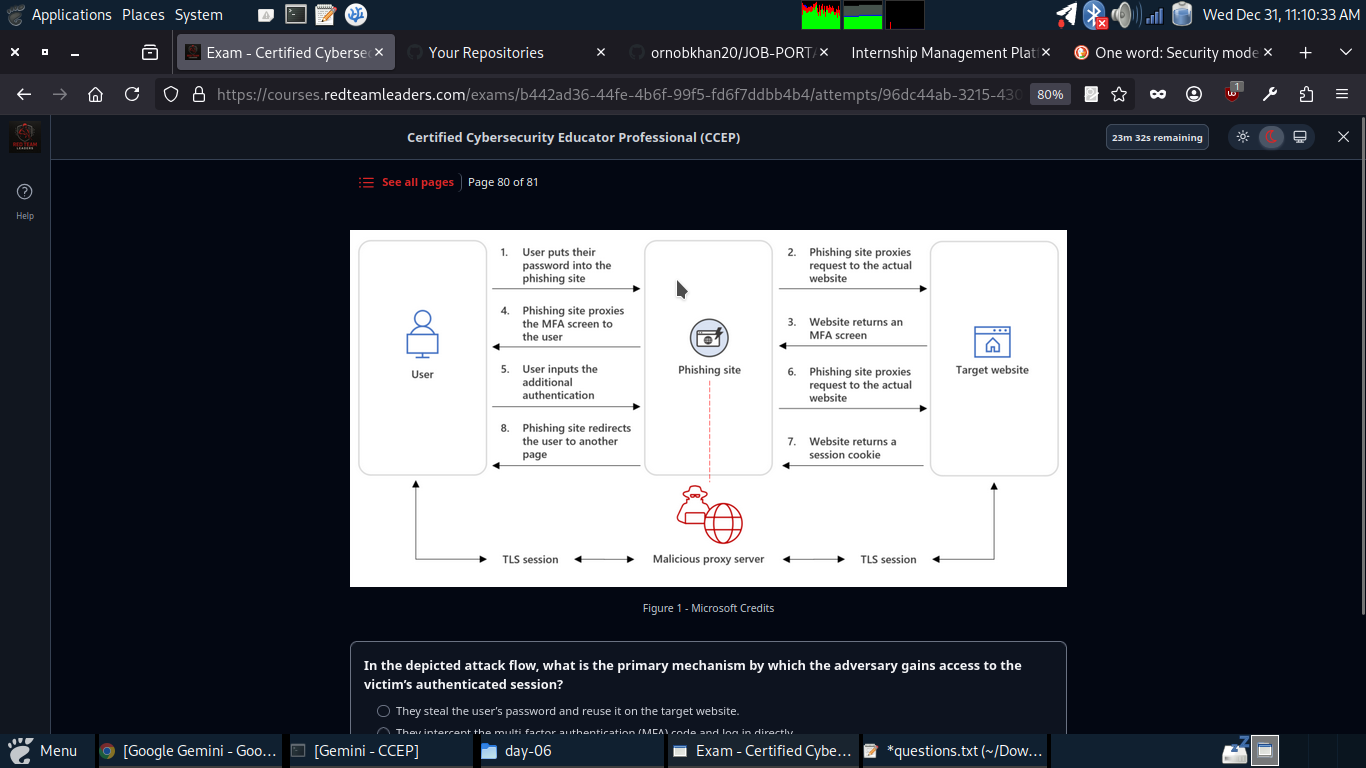
\includegraphics[width=0.5\linewidth]{./image001.png} % image scale = 0.5 of line width
	% 	\captionof{figure}{Image Caption that can be cited later}
	% \end{center}
	% some say \cite{doe2020signal} and \cite{smithe2019quantum}
	% There are some very deep faults in the entire REACT system \cite{the_react_team_denial_2025} which we could not solve due to lack on knowledge and the solution not yet properly defined and documented.
	
	
	\bibliographystyle{IEEEtran}
	\bibliography{./reference/reference.bib}
\end{document}